%!TEX TS-program = lualatex
%!TEX encoding = UTF-8 Unicode

\documentclass[12pt]{article}
\usepackage{graphicx}
	\graphicspath{{/Users/goby/Pictures/teach/163/lab/}
	{img/}} % set of paths to search for images

\usepackage{geometry}
\geometry{letterpaper, left=1in, bottom=0.5in, top=1in, right=0.5in}                   
\geometry{landscape}                % Activate for for rotated page geometry
\usepackage[parfill]{parskip}    % Activate to begin paragraphs with an empty line rather than an indent
%\usepackage{amssymb, amsmath}
%\usepackage{mathtools}
%	\everymath{\displaystyle}

\usepackage{fontspec}
\setmainfont[Ligatures={TeX}, BoldFont={* Bold}, ItalicFont={* Italic}, BoldItalicFont={* BoldItalic}, Numbers={OldStyle}]{Linux Libertine O}
\setsansfont[Scale=MatchLowercase,Ligatures=TeX]{Linux Biolinum O}
\setmonofont[Scale=MatchLowercase]{Linux Libertine Mono O}
\usepackage{microtype}


% To define fonts for particular uses within a document. For example, 
% This sets the Libertine font to use tabular number format for tables.
 %\newfontfamily{\tablenumbers}[Numbers={Monospaced}]{Linux Libertine O}
% \newfontfamily{\libertinedisplay}{Linux Libertine Display O}


\usepackage{tikz}

\usepackage[sc]{titlesec}


\newif\ifdates

\datestrue
%\datesfalse

\begin{document}

\thispagestyle{empty}

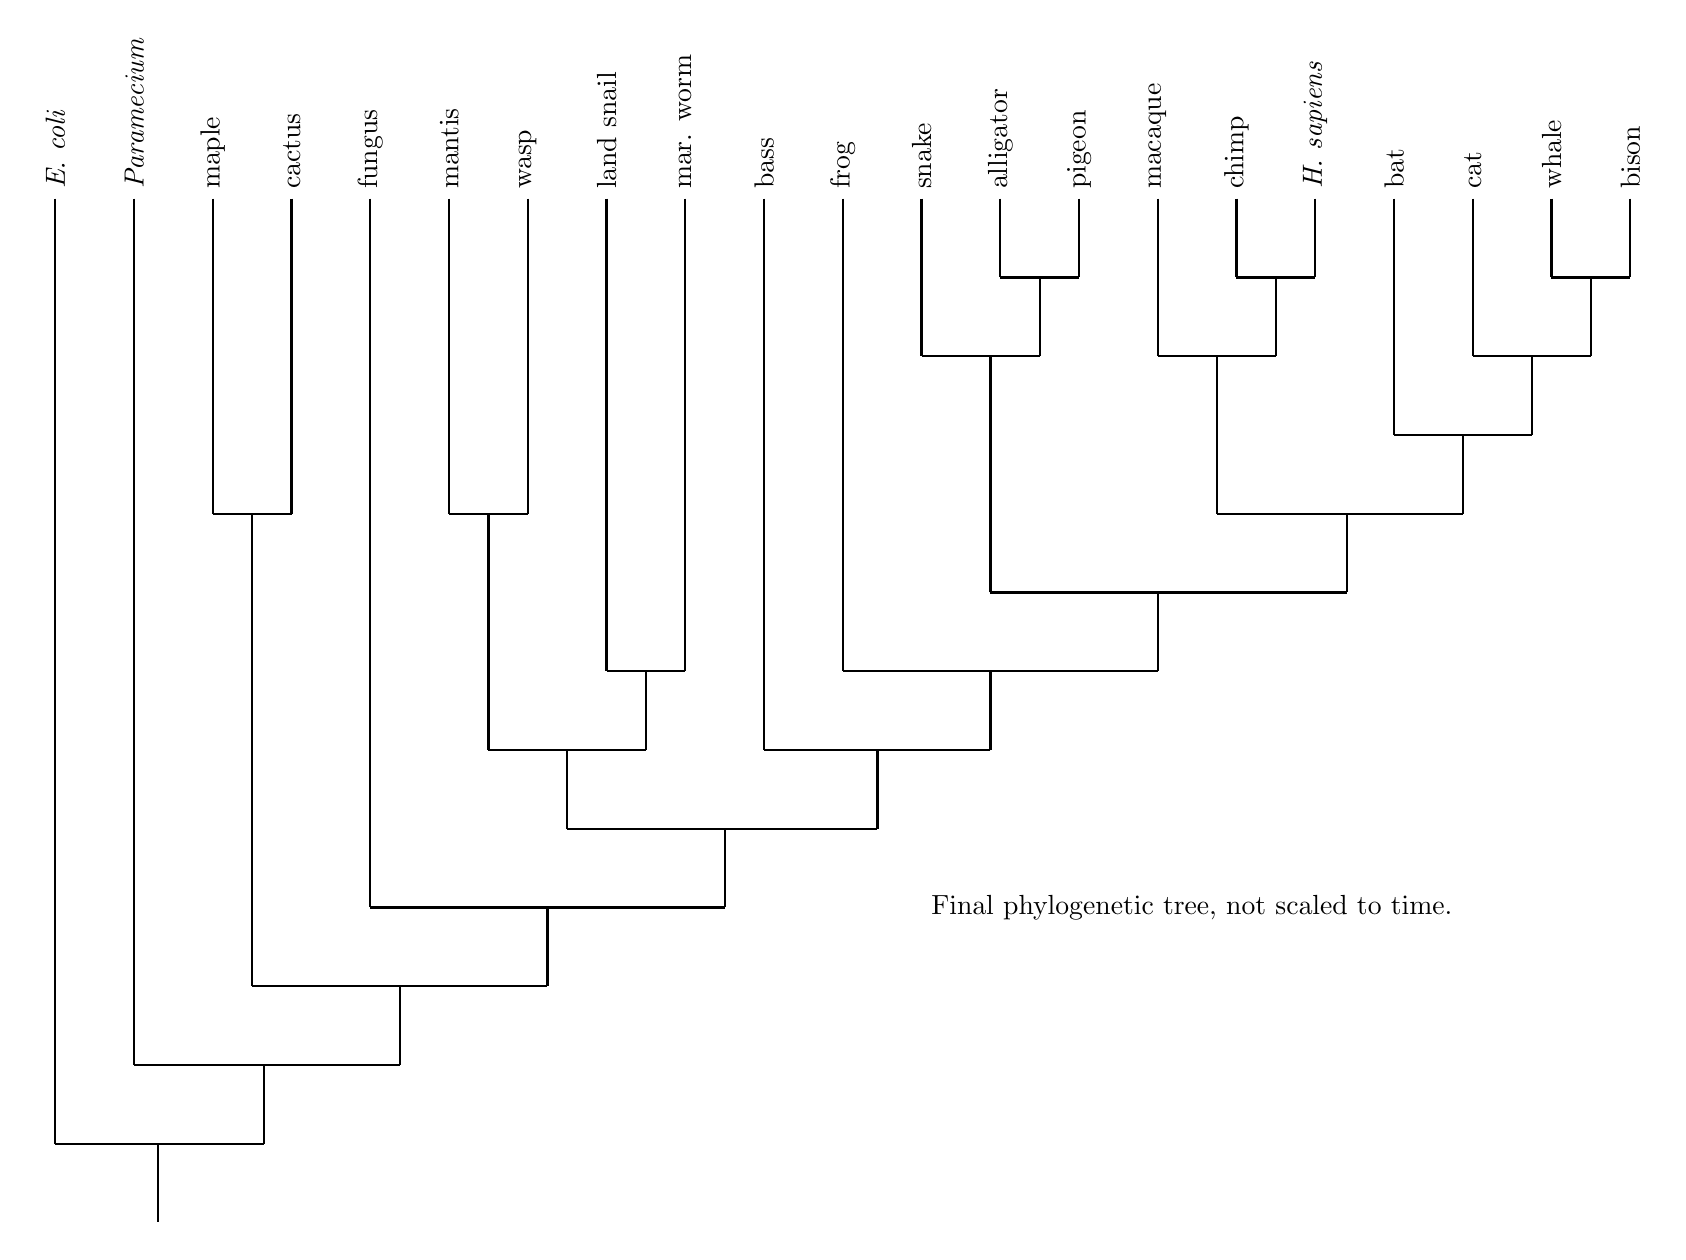
\begin{tikzpicture}

\tikzstyle{block} = [minimum size=2em, rotate=90, anchor=west]
\tikzstyle{branch} = [thick, draw]
%\tikzstyle{ancestor} = [anchor=center]

%\draw (0,0) [thick] -- coordinate (x axis mid) (22,0);

%\draw (0,0) [thick] -- coordinate (y axis mid) (0, 15);

%\foreach \y / \label in {0/8,1/7, 2/6, 3/5, 4/4, 5/3, 6/2, 7/1,8/0}
%	\draw [yscale=1.5] (1pt, \y) -- (-4pt,\y)
%		node[anchor=east] {\label};

%\node [rotate=90, above=0.8cm] at (y axis mid) {Genetic distance};

\node [block] at (1,15) (ecoli) {\textit{E. coli}};
\node [block] at (2,15) (paramecium) {\textit{Paramecium}};
\node [block] at (3,15) (maple) {maple};
\node [block] at (4,15) (cactus) {cactus};
\node [block] at (5,15) (fungus) {fungus};
\node [block] at (6,15) (mantis) {mantis};
\node [block] at (7,15) (wasp) {wasp};
\node [block] at (8,15) (snail) {land snail};
\node [block] at (9,15) (worm) {mar. worm};
\node [block] at (10,15) (bass) {bass};
\node [block] at (11,15) (frog) {frog};
\node [block] at (12,15) (snake) {snake};
\node [block] at (13,15) (alligator) {alligator};
\node [block] at (14,15) (pigeon) {pigeon};
\node [block] at (15,15) (macaque) {macaque};
\node [block] at (16,15) (chimp) {chimp};
\node [block] at (17,15) (human) {\textit{H. sapiens}};
\node [block] at (18,15) (bat) {bat};
\node [block] at (19,15) (cat) {cat};
\node [block] at (20,15) (whale) {whale};
\node [block] at (21,15) (bison) {bison};

% Whale Bison Level 14
\node (whale_anc) at (20,14){};
\node (bison_anc) at (21,14){};
\node (whalebison_split) at (20.5, 14){};
\draw [branch] (whale) -- (whale_anc.center);
\draw [branch] (bison) -- (bison_anc.center);
\draw [branch] (bison_anc.center) -- (whale_anc.center);

% Add cat Level 13
\node (cat_anc) at (19,13){};
\node (whalebison) at (20.5, 13){};
\draw [branch] (cat) -- (cat_anc.center);
\draw [branch] (whalebison.center) -- (whalebison_split.center);
\draw [branch] (whalebison.center) -- (cat_anc.center);

%add bat Level 12
\node (bat_anc) at (18, 12) {};
\node[label = below left:  \ifdates 33\fi] (catwhale_split) at (19.75, 13) {};
\node (catwhale_anc) at (19.75, 12) {};

\draw [branch] (bat) -- (bat_anc.center);
\draw [branch] (catwhale_split.center) -- (catwhale_anc.center);
\draw [branch] (bat_anc.center) -- (catwhale_anc.center);

% Human chimp level 14
\node (human_anc) at (17,14){};
\node (chimp_anc) at (16,14){};
\draw [branch] (chimp) -- (chimp_anc.center);
\draw [branch] (human) -- (human_anc.center);
\draw [branch] (chimp_anc.center) -- (human_anc.center);

% Add macaque level 13
\node (macaque_anc) at (15,13){};
\node [label = below left: \ifdates 5\fi] (humanchimp_split) at (16.5, 14){};
\node (humanchimp_anc) at (16.5, 13){};

\draw [branch] (macaque) -- (macaque_anc.center);
\draw [branch] (humanchimp_split.center) -- (humanchimp_anc.center);
\draw [branch] (macaque_anc.center) -- (humanchimp_anc.center);

% Mammals, level 11

\node [label = below left: \ifdates 52\fi](batcat_split) at (18.875, 12){};
\node (batcat_anc) at (18.875, 11){};
\node [label = below left: \ifdates 33\fi](macchimp_split) at (15.75, 13){};
\node (macchimp_anc) at (15.75, 11){};

\draw [branch] (batcat_split.center) -- (batcat_anc.center);
\draw [branch] (batcat_anc.center) -- (macchimp_anc.center);
\draw [branch] (macchimp_split.center) -- (macchimp_anc.center);

% Alligator pigeon level 14
\node (alligator_anc) at (13,14){};
\node (pigeon_anc) at (14, 14){};

\draw [branch] (alligator) -- (alligator_anc.center);
\draw [branch] (pigeon) -- (pigeon_anc.center);
\draw [branch] (pigeon_anc.center) -- (alligator_anc.center);

% Add snake, level 13
\node (snake_anc) at (12,13){};
\node [label = below left: \ifdates 200\fi](allipig_split) at (13.5, 14){};
\node (allipig_anc) at (13.5, 13){};

\draw [branch] (snake) -- (snake_anc.center);
\draw [branch] (allipig_split.center) -- (allipig_anc.center);
\draw [branch] (allipig_anc.center) -- (snake_anc.center);

% Amniotes10
\node (pigsnake_split) at (12.875, 13){};
\node (pigsnake_anc) at (12.875,10){};
\node [label = below left: \ifdates 290\fi](mammal_split) at (17.4,11){};
\node (mammal_anc) at (17.4,10){};

\draw [branch] (pigsnake_anc.center) -- (pigsnake_split.center);
\draw [branch] (mammal_split.center) -- (mammal_anc.center);
\draw [branch] (mammal_anc.center) -- (pigsnake_anc.center);

% Add frog, level 9
\node [label = below left: \ifdates 325\fi](amniote_split) at (15, 10){};
\node (amniote_anc) at (15 ,9){};
\node (frog_anc) at (11,9) {};

\draw [branch] (amniote_split.center) -- (amniote_anc.center);
\draw [branch] (frog) -- (frog_anc.center);
\draw [branch] (frog_anc.center) -- (amniote_anc.center);

% Add bass level 8
\node [label = below left: \ifdates 354\fi](tetrapod_split) at (12.875, 9){};
\node (tetrapod_anc) at (12.875, 8){};
\node (bass_anc) at (10, 8){};

\draw [branch] (bass) -- (bass_anc.center);
\draw [branch] (tetrapod_split.center) -- (tetrapod_anc.center);
\draw [branch] (tetrapod_anc.center) -- (bass_anc.center);


% MarWorm Snail, level 14
\node (worm_anc) at (9,9){};
\node (snail_anc) at (8,9){};
\node [label = below left: \ifdates 354\fi](wormsnail_split) at (8.5, 9){};
\draw [branch] (worm) -- (worm_anc.center);
\draw [branch] (snail) -- (snail_anc.center);
\draw [branch] (snail_anc.center) -- (worm_anc.center);

% wasp mantis, level 14
\node (wasp_anc) at (7,11){};
\node (mantis_anc) at (6,11){};
\node [label = below: \ifdates 144 or 354\fi](waspmantis_split) at (6.5, 11){};

\draw [branch] (wasp) -- (wasp_anc.center);
\draw [branch] (mantis) -- (mantis_anc.center);
\draw [branch] (mantis_anc.center) -- (wasp_anc.center);

% inverts, level 13
\node (waspmantis_anc) at (6.5, 8){};
\node (wormsnail_anc) at (8.5, 8){};

\draw [branch] (waspmantis_anc.center) -- (waspmantis_split.center);
\draw [branch] (wormsnail_anc.center) -- (wormsnail_split.center);
\draw [branch] (waspmantis_anc.center) -- (wormsnail_anc.center);

% Animals level 7
\node [label = below left: \ifdates 443\fi](vert_split) at (11.44,8){};
\node (vert_anc) at (11.44, 7){};

\node [label = below left: \ifdates 443\fi](invert_split) at (7.5, 8) {};
\node (invert_anc) at (7.5, 7) {};

\draw [branch] (invert_split.center) -- (invert_anc.center);
\draw [branch] (vert_split.center) -- (vert_anc.center);
\draw [branch] (invert_anc.center) -- (vert_anc.center);

% Add fungus, level 6
\node (fungus_anc) at (5, 6){};
\node  [label = below left: \ifdates 543\fi](animal_split) at (9.5, 7){};
\node (animal_anc) at (9.5, 6){};

\draw [branch] (fungus) -- (fungus_anc.center);
\draw [branch] (animal_split.center) -- (animal_anc.center);
\draw [branch] (fungus_anc.center) -- (animal_anc.center);

% Maple Cactus Level 14
\node (cactus_anc) at (4,11){};
\node (maple_anc) at (3,11){};
\node [label = below: \ifdates 144 or 55\fi] (plant_split) at (3.5, 11){};

\draw [branch] (cactus) -- (cactus_anc.center);
\draw [branch] (maple) -- (maple_anc.center);
\draw [branch] (maple_anc.center) -- (cactus_anc.center);

% Multicellular, level 5
\node (plant_anc) at (3.5, 5){};
\node (fungan_split) at (7.25, 6){};
\node (fungan_anc) at (7.25, 5){};

\draw [branch] (fungan_split.center) -- (fungan_anc.center);
\draw [branch] (plant_split.center) -- (plant_anc.center);
\draw [branch] (plant_anc.center) -- (fungan_anc.center);

% Paramecium , level 4
\node (paramecium_anc) at (2, 4){};
\node (multi_anc) at (5.375, 4) {};
\node [label = below left: \ifdates 900\fi](multi_split) at (5.375, 5) {};

\draw [branch] (paramecium) -- (paramecium_anc.center);
\draw [branch] (multi_anc.center) -- (multi_split.center);
\draw [branch] (multi_anc.center) -- (paramecium_anc.center);

% Ecoli, level 3
\node (ecoli_anc) at (1, 3){};
\node [label = below left: \ifdates 1.6 \textsc{bya}\fi](eukary_split) at (3.65, 4){};
\node (eukary_anc) at (3.65, 3){};

\draw [branch] (ecoli) -- (ecoli_anc.center);
\draw [branch] (eukary_split.center) -- (eukary_anc.center);
\draw [branch] (ecoli_anc.center) -- (eukary_anc.center);

% Root, level 2

\node [label=below left: \ifdates 3.8 \textsc{bya}\fi] (all_split) at (2.3, 3){};
\node (root) at (2.3, 2){};

\draw [branch] (all_split.center) -- (root.center);

\node [anchor=west] at (12,6) {Final phylogenetic tree, not scaled to time.};
\ifdates \node [anchor=west] at (12,5) {All times millions of years ago except where noted as \textsc{bya}.};
\node [anchor=west] at (12,4) {Give leeway on times. It can be difficult to match some times to nodes.};
\fi

\end{tikzpicture}

\end{document}  